% !TEX encoding = windows-1250
\documentclass[12pt, oneside, a4paper]{mwbk}
\usepackage[cp1250]{inputenc}
\usepackage[polish]{babel}
\usepackage[OT4]{fontenc}

\usepackage{listings}
\lstset
{
	captionpos=b,
	basicstyle=\footnotesize\ttfamily,
	frame = single,
	tabsize = 3,
	breaklines = true
}
\renewcommand\lstlistlistingname{Spis listing�w}

\usepackage{graphicx}
\usepackage{verbatim}

\usepackage{enumitem}
\usepackage[noend]{algorithmic}
\usepackage[ruled]{algorithm}

\usepackage{color}
\usepackage[normalem]{ulem}

\usepackage{rotating}
\usepackage{float}
\usepackage{textpos}

\linespread{1,3}
\oddsidemargin = 10pt
\textwidth = 470pt

\hyphenpenalty=1000
\tolerance=500

\begin{document}
\author{Krzysztof Szczech}
\title{Tytu�}
\begin{titlepage}
\thispagestyle{empty}
\begin{textblock}{1}(-2.65,-1.65)

\includegraphics{figures/tytulowa_pusta_mgrinz.pdf}
\end{textblock}
\vspace{7.3cm}
\begin{center}
\fontfamily{ptm}
\selectfont
\Huge
Wybrane aspekty techniczne odwzorowania artystycznej wizji jako tr�jwymiarowego �rodowiska w grze komputerowej
\end{center}
\begin{center}
\fontfamily{ptm}
\selectfont
Praca dyplomowa in�ynierska
\end{center}
\vspace{5.6cm}
\begin{center}
\fontfamily{ptm}
\selectfont
\hspace{-1cm}
\begin{tabular}{l}
Wydzia� Fizyki Technicznej, Informatyki i Matematyki Stosowanej \\
Promotor: dr in�. Rafa� Szrajber \\
Dyplomant: Krzysztof Szczech \\
Nr albumu: 180707 \\
Kierunek: Informatyka \\
Specjalno��: Technologie gier i symulacji komputerowych
\end{tabular}
\end{center}
\vspace{-.5cm}
\begin{center}
\fontfamily{ptm}
\selectfont
\begin{textblock}{13}(0,0.2)
��d�, 2016
\end{textblock}
\end{center}
\end{titlepage}

\tableofcontents

% !TeX encoding = windows-1250

\chapter{Wst�p}
\label{t:int}
Bardzo szybki - trwaj�cy od kilku dziesi�cioleci - rozw�j komputer�w pozwoli� na przenoszenie coraz bardziej z�o�onych fragment�w otaczaj�cego nas �wiata na ekrany monitor�w. Jeste�my w stanie symulowa� skomplikowane zjawiska przyrody, co pozwala nam lepiej zrozumie� �wiat na kt�rym �yjemy, "budowa�"  wirtualne domy w kt�rych kiedy� b�dziemy chcieli zamieszka� w rzeczywisto�ci, czy te� tworzy� obrazy bez pomocy p��tna i p�dzla.\newline
W latach 90. XX wieku zacz�to tworzy� pierwsze gry komputerowe wykorzystuj�ce wielok�tow� grafik� tr�jwymiarow� [1]. By� to pocz�tek nowej ery dla elektronicznej rozrywki. Pocz�tkowo liczba wielok�t�w by�a niska, a obraz by� renderowany w niewielkiej rozdzielczo�ci. Wraz z pojawianiem si� nowych akcelerator�w 3D liczby te zacz�y si� zwi�ksza�, co poprawia�o og�ln� jako�� grafiki. \newline 
Jednak po dzi� dzie� - mimo znacz�cego skoku technologicznego - pozosta� problem optymalnego tworzenia modeli i tekstur do gier w taki spos�b, aby komputer by� w stanie wytworzy� odpowiedni� liczb� klatek obrazu na sekund�. Przez lata rozwoju silnik�w graficznych  prze�cigano si� w pomys�ach na to, jak tworzy� assety (tr�jwymiarowe modele, tekstury, materia�y i animacje) aby wygl�da�y jak najatrakcyjniej dla gracza i jednocze�nie ich wykorzystywanie wymaga�o jak najmniejszej ilo�ci zasob�w komputera - w szczeg�lno�ci pami�ci RAM karty graficznej. Przy �le rozplanowanym procesie tw�rczym mo�e doj�� do sytuacji w kt�rej znacznie wyd�u�y si� czas oczekiwania na wczytanie z dysku twardego wszystkich wymaganych plik�w lub - w bardziej skrajnych przypadkach - karta graficzna komputera nie b�dzie nad��a�a z odpowiednio szybkim wytwarzaniem klatek animacji - co w znacznym stopniu zmniejszy komfort rozgrywki oraz poziom imersji gracza. Odpowiedni balans mi�dzy wspomnianymi aspektami jest jednym z najwi�kszych wyzwa� przed jakimi stawiani s� tw�rcy grafiki komputerowej wykorzystywanej w grach. \newpage
\section{Cel i za�o�enia pracy}
Celem pracy jest przedstawienie procesu tworzenia paczki modeli oraz tekstur na podstawie grafiki koncepcyjnej, kt�re jednocze�nie s� gotowe do wykorzystania w silniku gry komputerowej. Dodatkowo - szczeg�lny nacisk zosta� po�o�ony na techniczne aspekty tego procesu - w szczeg�lno�ci jak najlepsze wykorzystanie pami�ci operacyjnej komputera. Aby osi�gn�� zamierzony cel, zaprojektowano proces wytwarzania modeli i tekstur dla wybranej technologii a nast�pnie wytworzono je, zaimportowano do silnika 3D oraz stworzono tr�jwymiarowy poziom przypominaj�cy ten z wybranej grafiki koncepcyjnej. Praca zawiera r�wnie� opisy wykorzystanych technik optymalizacji. \newline
Cel zrealizowano z wykorzystaniem nast�puj�cych narz�dzi:
\begin{description}
	\item[Silnik 3D:] \hfill \\ \textit{Unreal Engine 4} - wyb�r podyktowany przede wszystkim wykorzystywaniem przez niego bardzo zaawansowanych algorytm�w renderingu (physically based rendering) pozwalaj�cych na uzyskanie bardzo szczeg�owych i realistycznie odwzorowanych obraz�w oraz wcze�niejsz� znajomo�ci� tej technologii. Alternatywnym wyborem m�g�by by� silnik \textit{Unity 5} (r�wnie� implementuj�cy te algorytmy), \textit{CryEngine 3} lub dowolny inny silnik pozwalaj�cy na renderowanie tr�jwymiarowych obiekt�w (w��czaj�c r�wnie� w�asn� implementacj�)
	\item[Modelowanie 3D:] \hfill \\ \textit{Autodesk 3ds Max 2016} - zaawansowanie narz�dzie do tworzenia tr�jwymiarowych modeli. Zamiast niego mo�na r�wnie� wykorzysta� takie programy, jak: \textit{Autodesk Maya}, \textit{Cinema 4D}, czy darmowy dla komercyjnego u�ytku \textit{Blender}.
	\item[Teksturowanie:] \hfill \\ \textit{Adobe Photoshop CS6} - program do tworzenia i obr�bki dwuwymiarowej grafiki. \newline
	\textit{Crazy Bump} - narz�dzie pozwalaj�ce na tworzenie tekstur nier�wno�ci i szorstko�ci obiekt�w.
	\item[Dodatkowe narz�dzia:] \hfill \\ \textit{Microsoft Excel} - wykorzystywany w procesie planowania do wypisywania list wymaganych asset�w.
\end{description}
\section{Zakres pracy}
Zakres pracy obejmuje wykorzystanie wybranych 

% !TeX encoding = windows-1250
\begin{thebibliography}{999}
	\bibitem{MostInfluentialGames} 15 Most Influential Games of All Time, \emph{Virtua Racing � Arcade (1992)}, \newline\texttt{https://web.archive.org/web/20100412225953/http://www.gamespot.com/gamespot\newline/features/video/15influential/p13\_01.html}, witryna internetowa, stan na 28 lipca 2016
	
	\bibitem{Investigation} S. Jones, \emph{Investigation into modular design within computer games}, praca licencjacka, Uniwersytet Staffordshire, 2011
	
	\bibitem{CreatingModularGameArt} Creating Modular Game Art For Fast Level Design, \texttt{http://www.gamasutra.com/view/feature/130885\newline/creating\_modular\_game\_art\_for\_fast\_.php}, witryna internetowa, stan na 31 lipca 2016
\end{thebibliography}


\newpage
\thispagestyle{empty}
\begin{textblock}{1}(-2.65,-1.65)
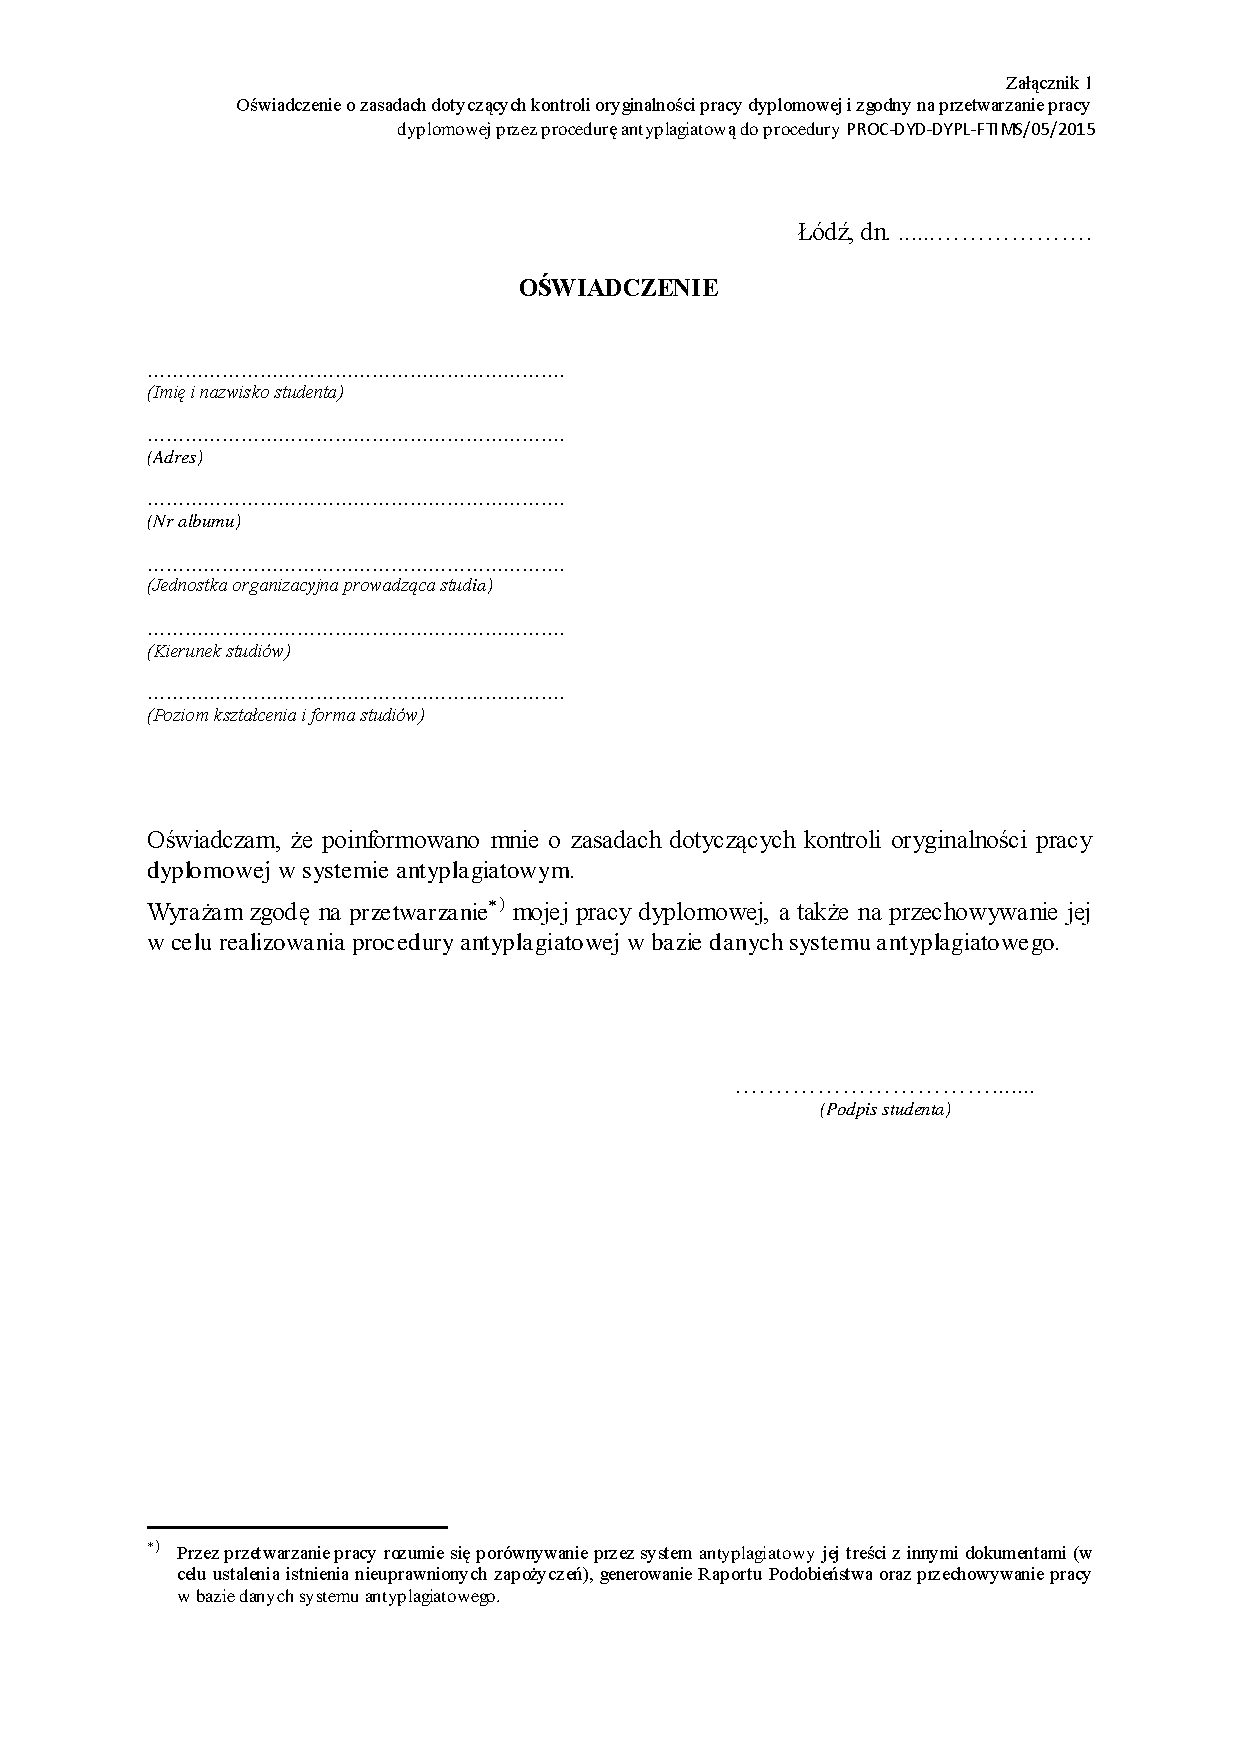
\includegraphics{figures/Zal_1.pdf}
\end{textblock}

\newpage
\thispagestyle{empty}
\begin{textblock}{1}(-2.65,-1.65)
	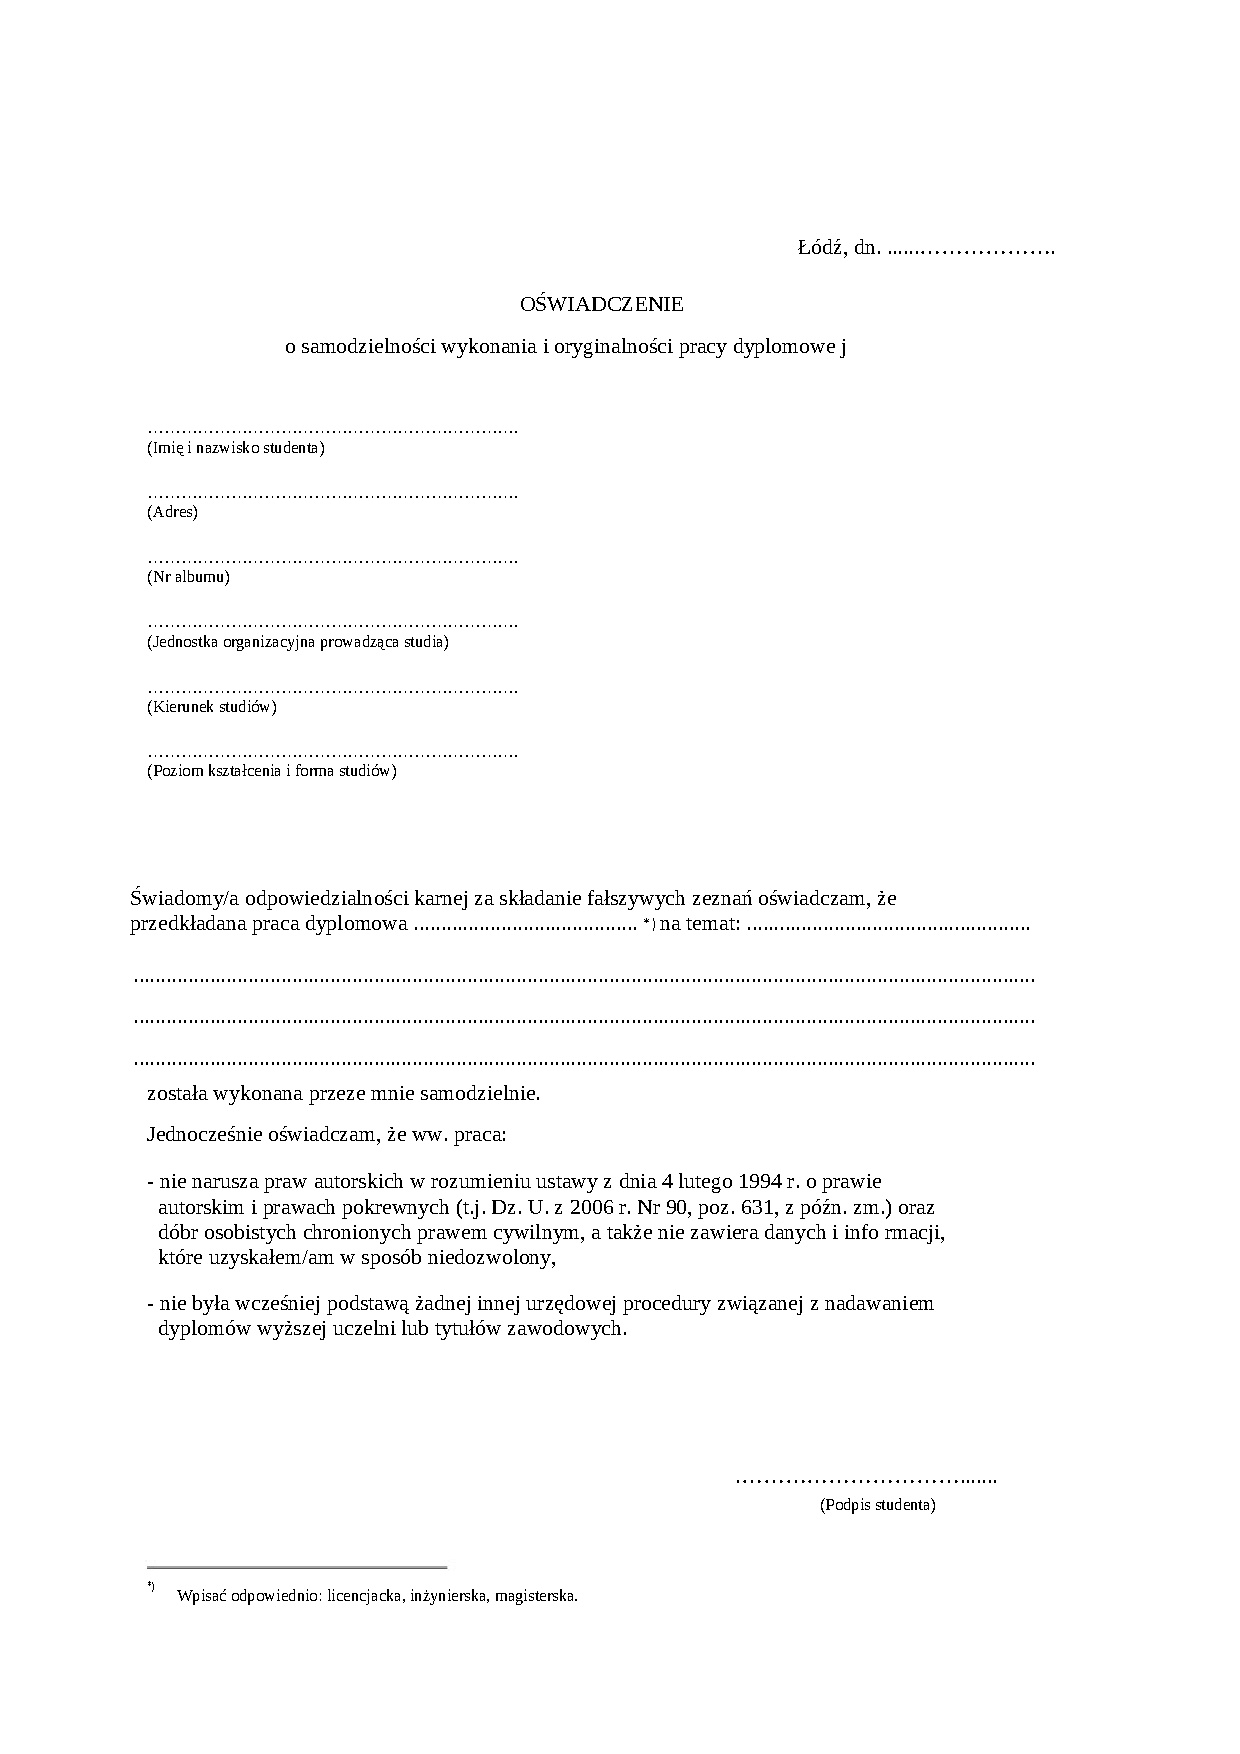
\includegraphics{figures/Zal_2.pdf}
\end{textblock}

\newpage
\thispagestyle{empty}
\begin{textblock}{1}(-2.65,-1.65)
	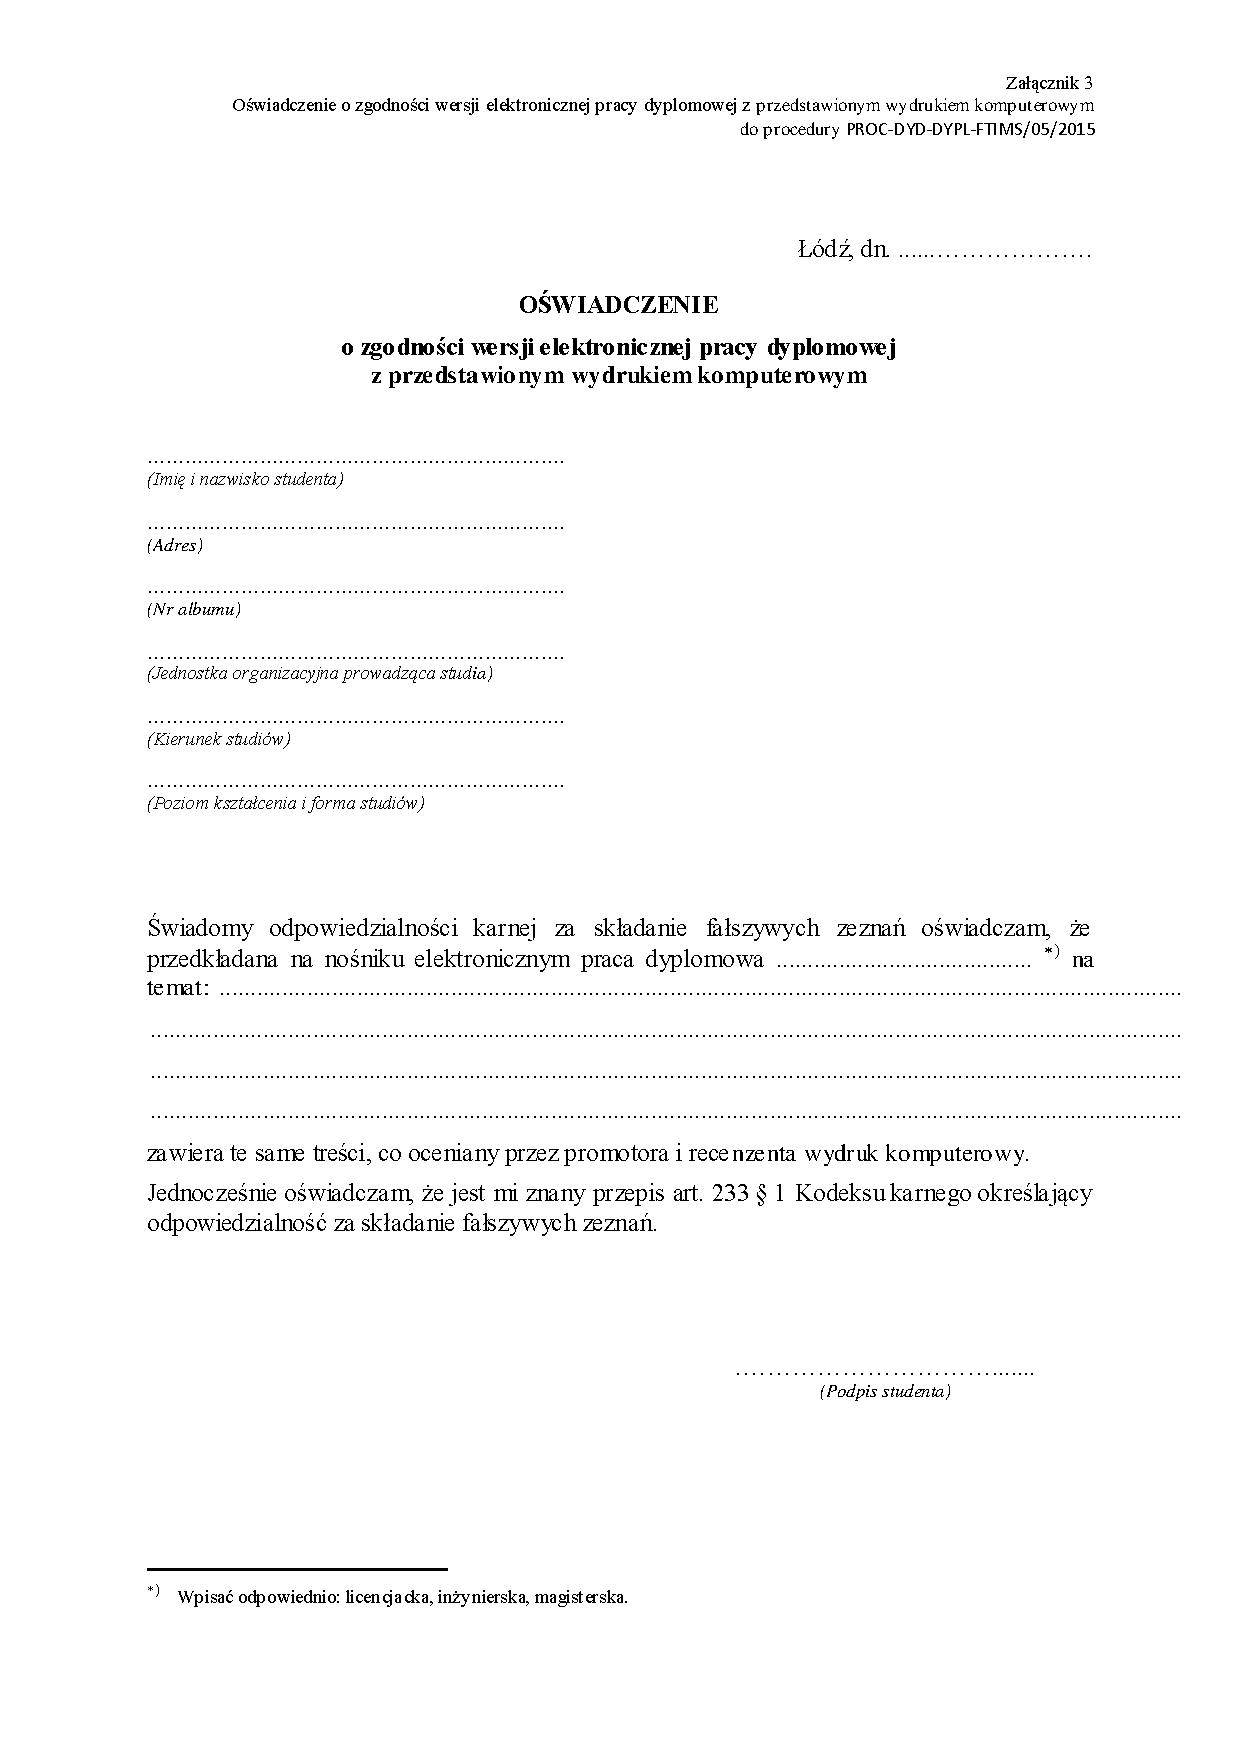
\includegraphics{figures/Zal_3.pdf}
\end{textblock}

\end{document}
